\section{Requirement and Data Analysis}
This project aims to develop a deep learning model for ECG heartbeat classification using the MIT-BIH Arrhythmia Dataset. The model should classify ECG heartbeats into five distinct categories while achieving a minimum accuracy of 95\% on the test dataset. Various AI models will be compared and evaluated based on key performance metrics, including accuracy, precision, recall, and F1-score. Additionally, the model must generalize well, avoid overfitting and ensure robustness on unseen ECG signals.

Considering computational constraints, training should be completed within five hours on an M2 MacBook Air. Furthermore, compliance with EU regulations regarding medical AI is essential, handling patient data is a sensitive issue, therefor compliance with GDPR is mandatory.

\subsection{Project Specifications}\label{sec:project-specs}
The project specifications are as follows:
\begin{enumerate}
    \item \textbf{Dataset:} MIT-BIH Arrhythmia Dataset (five heartbeat classes).
    \item \textbf{Accuracy Target:} $\geq$95\% classification accuracy on the MIT-BIH test dataset.
    \item \textbf{Training Time Constraint:} Training should not exceed five hours on an M2 MacBook Air.
    \item \textbf{Generalization:} The model should perform reliably on unseen ECG signals, minimizing overfitting.
    \item \textbf{Performance Metrics:} Evaluation based on accuracy, precision, recall, and F1-score.
\end{enumerate}

\subsection{Dataset Overview}
The dataset used in this project originates from Kaggle's ECG Heartbeat Categorization Dataset \cite{b1}, derived from the MIT-BIH Arrhythmia Dataset from PhysioNet. It consists of 109,446 ECG heartbeats labeled into five classes: Normal, Supraventricular, Ventricular, Fusion, and Unknown. The dataset is divided into:
\begin{itemize}
    \item \textbf{Training set:} 87,554 samples
    \item \textbf{Testing set:} 21,890 samples
\end{itemize}

The dataset exhibits class imbalance, with the Normal class having the highest number of samples, while the Fusion class has the least.

\subsection{Data Visualization}
To gain insight into the dataset, we visualize the class distribution and ECG heartbeat samples. Figure \ref{fig:original_trainset_distribution} presents the original training dataset distribution and fig \ref{fig:original_testset_distribution}, the, while Figure \ref{fig:ecg_samples} showcases representative ECG waveforms for each class selected randomly.

\begin{figure}[htbp]
    \centering
    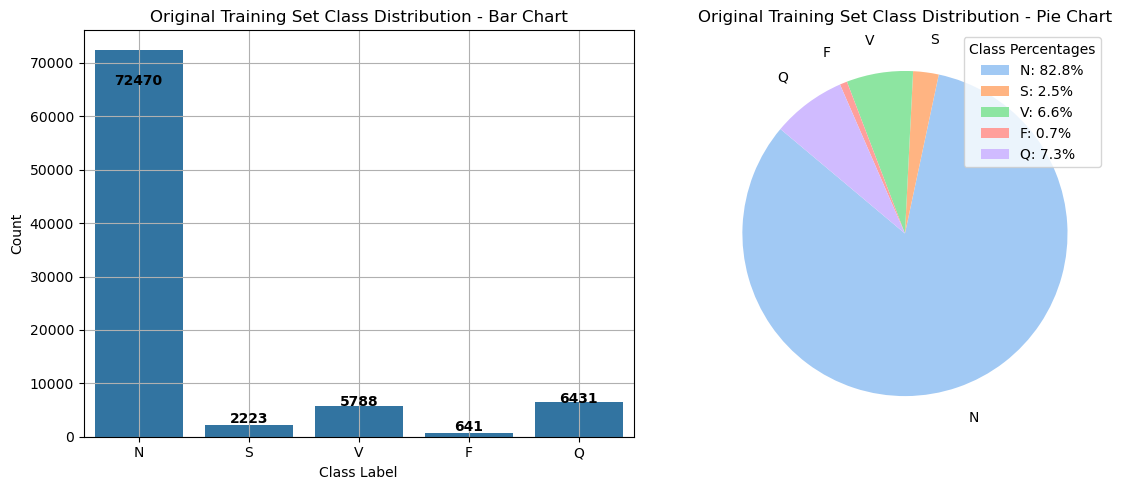
\includegraphics[width=0.5\textwidth]{images/OriginalDatasetTrainingDistribution.png}
    \caption{Original Trainng Dataset Distribution}
    \label{fig:original_trainset_distribution}
\end{figure}

\begin{figure}[htbp]
    \centering
    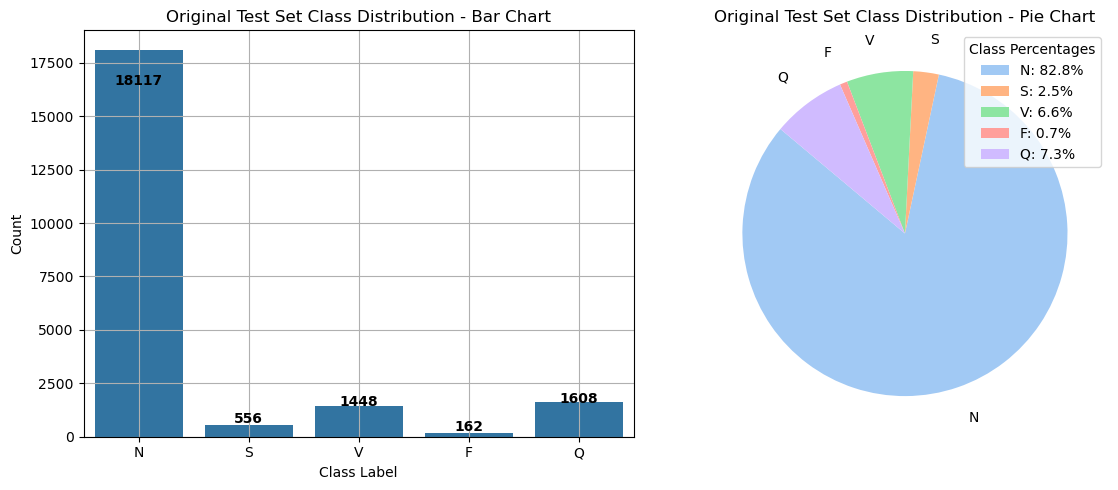
\includegraphics[width=0.5\textwidth]{images/OriginalDatasetTestDistribution.png}
    \caption{Original Test Dataset Distribution}
    \label{fig:original_testset_distribution}
\end{figure}

\begin{figure}[htbp]
    \centering
    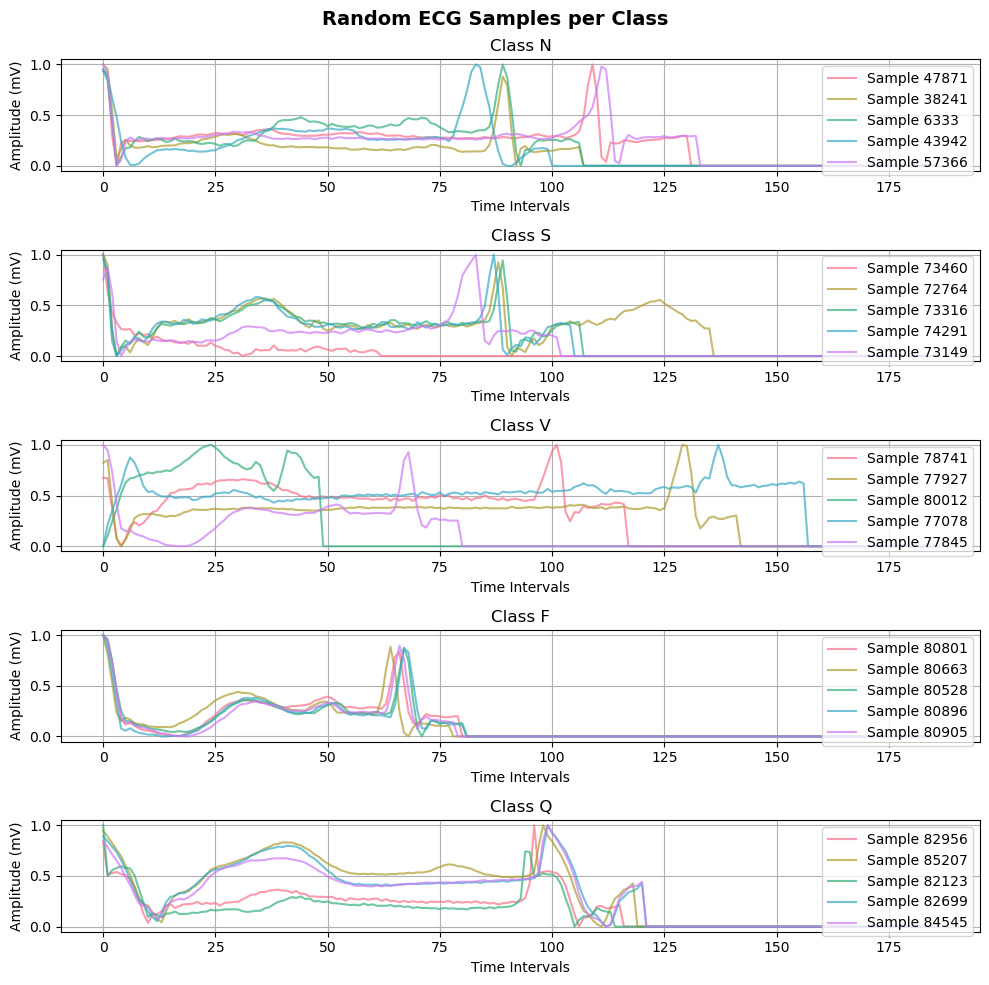
\includegraphics[width=0.5\textwidth]{images/RandomECGsamplesPerClass.png}
    \caption{ECG Heartbeat Samples}
    \label{fig:ecg_samples}
\end{figure}
